

In the US, we keep each of these facilities separate in the front-end of
the fuel cycle in a "collect and wait" pathway \cite{cycle_risks}. In
lieu of a long or interim solution for the \gls{uf}, the back end of the
\gls{nfc} is collocated with the reactors that burn the fuel (with the
minor exception of the consolidated storage facility in Morris Illinois).

Nuclear fuel has the capacity to be
reprocessed and recycled into a different fuel type that can produce
usable power for several cycles, called a "closed" fuel cycle.





 \begin{figure}[h]
    \centering
    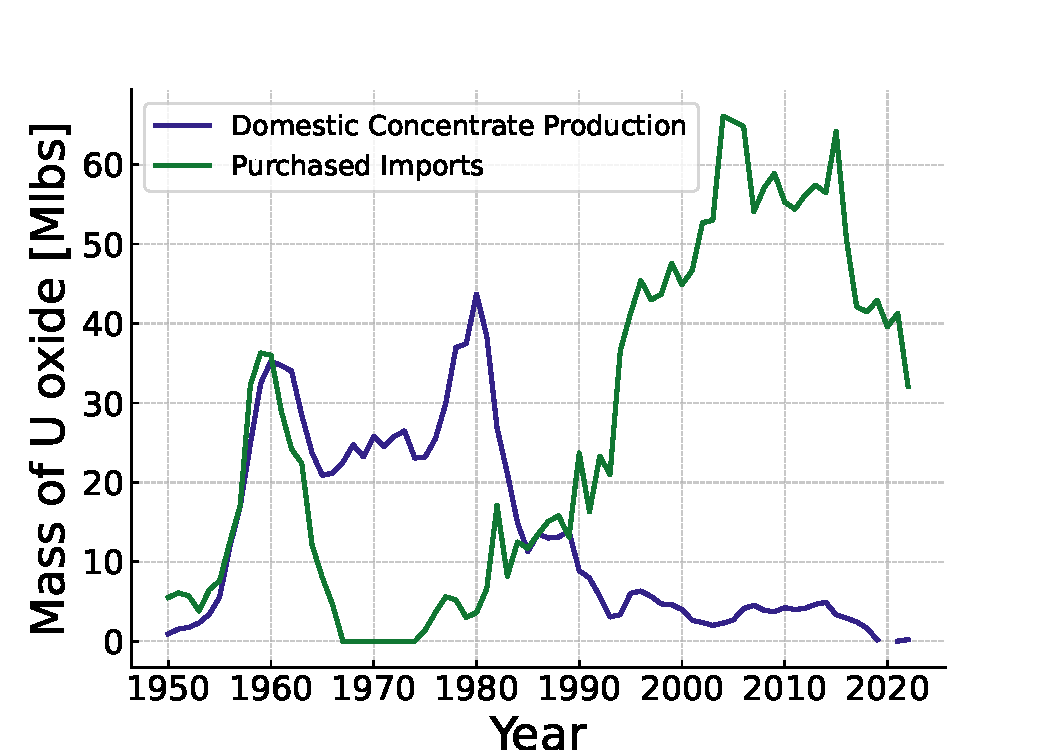
\includegraphics[scale=0.8]{images/intro/uranium_production_imports.pdf}
    \caption{Foregin and domestic uranium purchases over time \cite{eia_monthly_energy_review_2024}.}
    \label{fig:foregin_u3o8}
 \end{figure}